%%
%% This is file `sample-sigconf.tex',
%% generated with the docstrip utility.
%%
%% The original source files were:
%%
%% samples.dtx  (with options: `sigconf')
%% 
%% IMPORTANT NOTICE:
%% 
%% For the copyright see the source file.
%% 
%% Any modified versions of this file must be renamed
%% with new filenames distinct from sample-sigconf.tex.
%% 
%% For distribution of the original source see the terms
%% for copying and modification in the file samples.dtx.
%% 
%% This generated file may be distributed as long as the
%% original source files, as listed above, are part of the
%% same distribution. (The sources need not necessarily be
%% in the same archive or directory.)
%%
%%
%% Commands for TeXCount
%TC:macro \cite [option:text,text]
%TC:macro \citep [option:text,text]
%TC:macro \citet [option:text,text]
%TC:envir table 0 1
%TC:envir table* 0 1
%TC:envir tabular [ignore] word
%TC:envir displaymath 0 word
%TC:envir math 0 word
%TC:envir comment 0 0
%%
%%
%% The first command in your LaTeX source must be the \documentclass command.
\documentclass[sigconf]{acmart}

\usepackage{graphicx}
\usepackage{epsfig}
\usepackage{tikz}
\def\checkmark{\tikz\fill[scale=0.4](0,.35) -- (.25,0) -- (1,.7) -- (.25,.15) -- cycle;} 

%%
%% \BibTeX command to typeset BibTeX logo in the docs
\AtBeginDocument{%
  \providecommand\BibTeX{{%
    Bib\TeX}}}

%% Rights management information.  This information is sent to you
%% when you complete the rights form.  These commands have SAMPLE
%% values in them; it is your responsibility as an author to replace
%% the commands and values with those provided to you when you
%% complete the rights form.
\setcopyright{acmcopyright}
\copyrightyear{2023}
\acmYear{2023}
\setcopyright{rightsretained}
\acmConference[WWW '23]{Proceedings of the ACM Web Conference
2023}{May 1--5, 2023}{Austin, TX, USA}
\acmBooktitle{Proceedings of the ACM Web Conference 2023 (WWW '23),
May 1--5, 2023, Austin, TX, USA}
\acmDOI{10.1145/3543507.3583414}
\acmISBN{978-1-4503-9416-1/23/04}


%%
%% Submission ID.
%% Use this when submitting an article to a sponsored event. You'll
%% receive a unique submission ID from the organizers
%% of the event, and this ID should be used as the parameter to this command.
%%\acmSubmissionID{123-A56-BU3}

%%
%% For managing citations, it is recommended to use bibliography
%% files in BibTeX format.
%%
%% You can then either use BibTeX with the ACM-Reference-Format style,
%% or BibLaTeX with the acmnumeric or acmauthoryear sytles, that include
%% support for advanced citation of software artefact from the
%% biblatex-software package, also separately available on CTAN.
%%
%% Look at the sample-*-biblatex.tex files for templates showcasing
%% the biblatex styles.
%%

%%
%% The majority of ACM publications use numbered citations and
%% references.  The command \citestyle{authoryear} switches to the
%% "author year" style.
%%
%% If you are preparing content for an event
%% sponsored by ACM SIGGRAPH, you must use the "author year" style of
%% citations and references.
%% Uncommenting
%% the next command will enable that style.
%%\citestyle{acmauthoryear}



%%
%% end of the preamble, start of the body of the document source.
\begin{document}

%%
%% The "title" command has an optional parameter,
%% allowing the author to define a "short title" to be used in page headers.
\title{Hidden Indicators of Collective Intelligence in Crowdfunding}

%%
%% The "author" command and its associated commands are used to define
%% the authors and their affiliations.
%% Of note is the shared affiliation of the first two authors, and the
%% "authornote" and "authornotemark" commands
%% used to denote shared contribution to the research.

\author{Em\H oke-\'Agnes Horv\'at}
\affiliation{%
  \institution{Northwestern University}
  \streetaddress{2240 Campus Drive}
  \city{Evanston, IL}
  \country{USA}}
\email{a-horvat@northwestern.edu}

\author{Henry K. Dambanemuya}
\affiliation{%
  \institution{Northwestern University}
  \streetaddress{2240 Campus Drive}
  \city{Evanston, IL}
  \country{USA}}
\email{hdambane@u.northwestern.edu}

\author{Jayaram Uparna}
\affiliation{%
  \institution{Indian Institute of Management Udaipur}
  \streetaddress{ Balicha Campus}
  \city{Udaipur}
  \country{India}}
\email{jayaram.uparna@iimu.ac.in}

\author{Brian Uzzi}
\affiliation{%
  \institution{Northwestern University}
  \streetaddress{2211 Campus Drive}
  \city{Evanston, IL}
  \country{USA}}
\email{uzzi@kellogg.northwestern.edu}


%%
%% By default, the full list of authors will be used in the page
%% headers. Often, this list is too long, and will overlap
%% other information printed in the page headers. This command allows
%% the author to define a more concise list
%% of authors' names for this purpose.
\renewcommand{\shortauthors}{Horv\'at et al.}

%%
%% The abstract is a short summary of the work to be presented in the
%% article.
\begin{abstract}
Extensive literature argues that crowds possess essential collective intelligence benefits that allow superior decision-making by untrained individuals working in low-information environments. Classic wisdom of crowds theory is based on evidence gathered from studying large groups of diverse and independent decision-makers. Yet, most human decisions are reached in online settings of interconnected like-minded people that challenge these criteria. This observation raises a key question: Are there surprising expressions of collective intelligence online? Here, we explore whether crowds furnish collective intelligence benefits in crowdfunding systems. Crowdfunding has grown and diversified quickly over the past decade, expanding from funding aspirant creative works and supplying pro-social donations to enabling large citizen-funded urban projects and providing commercial interest-based unsecured loans. Using nearly 10 million loan contributions from a market-dominant lending platform, we find evidence for collective intelligence indicators in crowdfunding. Our results, which are based on a two-stage Heckman selection model, indicate that opinion diversity and the speed at which funds are contributed predict who gets funded and who repays, even after accounting for traditional measures of creditworthiness. Moreover, crowds work consistently well in correctly assessing the outcome of high-risk projects. Finally, diversity and speed serve as early warning signals when inferring fundraising based solely on the initial part of the campaign. Our findings broaden the field of crowd-aware system design and inform discussions about the augmentation of traditional financing systems with tech innovations.
\end{abstract}

%%
%% The code below is generated by the tool at http://dl.acm.org/ccs.cfm.
%% Please copy and paste the code instead of the example below.
%%
\begin{CCSXML}
<ccs2012>
   <concept>
       <concept_id>10003120.10003130.10011762</concept_id>
       <concept_desc>Human-centered computing~Empirical studies in collaborative and social computing</concept_desc>
       <concept_significance>500</concept_significance>
       </concept>
   <concept>
       <concept_id>10003120.10003121.10011748</concept_id>
       <concept_desc>Human-centered computing~Empirical studies in HCI</concept_desc>
       <concept_significance>500</concept_significance>
       </concept>
 </ccs2012>
\end{CCSXML}

\ccsdesc[500]{Human-centered computing~Empirical studies in collaborative and social computing}
\ccsdesc[500]{Human-centered computing~Empirical studies in HCI}

%%
%% Keywords. The author(s) should pick words that accurately describe
%% the work being presented. Separate the keywords with commas.
\keywords{crowds, collective decision-making, opinion diversity, aggregation speed, early warning signals}

%%
%% This command processes the author and affiliation and title
%% information and builds the first part of the formatted document.
\maketitle

\section{Introduction}
An impactful discovery in decision-making research has been ``crowd wisdom,'' or the ability of the crowd to make better decisions than individuals make~\cite{arrow2008promise,hertwig2012tapping,malone2010collective, woolley2010,woolley2015,gloor2006swarm}. Recent research has begun exploring the important question of whether the wisdom of crowds operates in complex human decision-making situations~\cite{mann2017optimal,moore2017confidence,prelec2017solution,guilbeault2020networked,becker2019wisdom,qiu2019crowd,samiotis2022scriptoria,da2020harnessing}. Currently, the wisdom of crowds studies show that crowds can produce better estimates of \emph{unknown knowns}---decisions where true answers are known a priori but not by the crowd. The original case of unknown knowns dating back to the early twentieth century involved guessing the weight of a quartered ox at an English countryside fair. The closest guesser would win the quartered ox. Only the butcher knew the ox’s true weight. The remarkable discovery was that the crowd’s estimate of the ox’s weight was better than any person's in the crowd, including people with expertise in cattle ranching and butchery. The crowd’s guessed weight, measured as the average of all guesses, was off by just 11 pounds (the true weight was 1109 pounds)~\cite{galton1907vox}. The power of crowds to guess unknown knowns has been replicated in diverse contexts~\cite{surowiecki2005wisdom,simoiu2019studying}, including estimating the number of jellybeans in a jar~\cite{becker2017network}.

In contrast to unknown knowns, complex decisions involve estimating \emph{unknown unknowns}, where the true value becomes known in the future instead of at the time of the guess\footnote{We argue that unknown unknowns are a crucial challenge in crowd decision-making, just as they are a weak spot in machine learning. In the case of machine learning, unknown unknowns represent examples where a model is confident about its answer but is wrong, as opposed to signaling that it is unsure of the answer~\cite{sharifi2022should,zhao2021exploratory,lakkaraju2017identifying}. Work in human computation demonstrates that humans can identify unknown unknowns in machine learning models, recognizing rare but important errors~\cite{attenberg2011beat}. Motivated by this evidence, we go one step further and use the concept of unknown unknowns to distinguish the toughest problems for collective intelligence that do not have a clear true value at the time of estimation. Specifically, our paper tests the ability of the crowd to provide superior decisions in complex real-world unknown unknowns.}. Complex decisions are widespread and include judgments about investments, patients’ reactions to therapies, the impact of climate on migration, insurance risks, mission failure, or the replicability of scientific findings~\cite{budescu2015identifying,chen2014wisdom,dreber2015using}. Typically, complex decision-making is left to specially trained or experienced experts~\cite{tetlock2017expert}. However, there is increasing evidence that expert decision-makers are more inaccurate and biased than was previously assumed~\cite{moore2017confidence,bonabeau2009decisions,tetlock2017expert}. Celebrated experts are barely more accurate than informed non-experts and, depending on the circumstances, as low as 12\% of the outcomes they predict actualize~\cite{tetlock2017expert,bonabeau2009decisions,moore2017confidence}. This suggests that the exploration of crowd wisdom for complex decision-making has both theoretical and practical importance~\cite{moore2017confidence}. Together, the limitations of expertise and the remarkable estimation accuracy of crowds raise new questions about whether crowd wisdom can provide decision-making support for complex decisions.  

Web systems enable broad tests of crowd wisdom’s potential application in complex decision-making. A growing area of crowd decision-making includes crowdfunding decisions, which is an important scientific study on its own~\cite{mollick2014dynamics,sorenson2016expand,gerber2013crowdfunding}. Over the past years, crowdfunding has grown rapidly in popularity, with some projecting that the global crowdfunding market will reach USD 28.9 billion by 2028~\cite{marketgrowth}. Crowdfunding could be especially critical in sectors under-served by traditional financing institutions~\cite{makina2019potential,arvila2020enabling}. Our analysis studies investment decision-making on one of the first crowdfunding platforms for personal loans in the U.S. Crowdfunding involves untrained novices making complex decisions about loaning their funds. Funds are loaned to anonymous borrowers who promise to repay the loan's principle with interest but who pledge no collateral in the event of default, meaning that the crowd bears the entire risk associated with financing. In crowdfunding, loan decisions rely on collective intelligence because the crowd agrees without the aid of a leader or formal organizational rules to fund or not fund the loan.

Collective intelligence is linked to a crowd’s diversity of opinions and the speed at which opinions are aggregated. When estimates are diverse, there is a greater likelihood that they will be equivalently dispersed above and below the true value, thereby averaging out estimation errors~\cite{Hong2004,Page2007}. When opinions arrive quickly, one after the other, the increased aggregation speed enables novel or specialized knowledge to be incorporated early into the crowd’s decisions, thus avoiding bias toward lowest common denominator information~\cite{surowiecki2005wisdom,lyon2013wisdom,prelec2017solution}. How these factors operate in complex decision situations involving unknown unknowns is unclear because unknown unknowns have no a priori true value, and decision-makers are predisposed to social influence~\cite{cialdini2006influence}. Experiments indicate that when individuals find it difficult to evaluate an object's true quality, they are susceptible to herding, which restricts the diversity of opinions~\cite{Salganik2006}. Similarly, fast aggregation can emphasize the first few estimates of quality, which can lead to collective decisions that are biased~\cite{Muchnik2013,Bikhchandani1992,Easley2010}.

We hypothesize that diversity and speed positively relate to prediction accuracy in real-world decisions but with a contingency. Because real-world decisions are complex and concern unknown unknowns, the mechanisms that generate collective intelligence need to be stronger for such decisions than they would need to be when the crowd is estimating unknown knowns. This suggests that the collective intelligence of the crowd for complex decisions with unknown unknowns requires both a high level of diversity and high speed for accurate collective decision-making. If either or both of these collective intelligence indicators are low, the crowd's decisions will be no more accurate than what is expected by the simple base rate. Specifically, we test whether crowds make accurate funding decisions as predicted by the diversity of opinion and the speed at which people collectively bid on a loan. A related theoretical and practical test is whether a few people reach the same decision as large groups in complex real-world estimation settings~\cite{navajas2018aggregated}. Due to their size, large crowds are intuitively likely to be more diverse and have more novel information. This raises the question of whether diversity and speed based on the first few contributors only (i.e., a small crowd) are associated with the funding decisions that large crowds made.

This paper thus puts to the test two non-trivial collective intelligence indicators (diversity and speed), finding empirically that they may benefit lenders and borrowers alike by promoting strategies for timely reinvesting and campaign retraction to avoid credit deterioration. Conceptually, our work identifies a compelling example of collective intelligence working better in practice than theories have predicted. In the human computation community, our findings call for concerted efforts to develop new theories of the wisdom of crowds that are inspired by parallel research in Web-enabled collective intelligence systems.

\begin{figure}
    \centering
     \includegraphics[scale=.25]{samples/figs/lending-amount.png}
    \includegraphics[scale=.25]{samples/figs/lending-time.png}
    \includegraphics[scale=.5]{samples/figs/lending-examples.png}
    \caption{Histograms of (a) contribution amounts and (b) inter-bid times. Evolution of campaigns on the lending platform (c): the raised capital as the percentage of the target amount is shown in function of time for successful and unsuccessful campaigns (depicted in tones of red and gray, respectively).}
    \label{fig:trajectories}
    \vspace{-2em}
\end{figure}

\section{Related Work}
The idea of human computation as a means to solving computational problems in crowdsourcing applications has attracted substantial research attention from diverse fields, including artificial intelligence and human-computer interaction (HCI)~\cite{quinn2011human}. Relatedly, the notion that large groups of loosely organized people can arrive at solutions superior to those invented by any individual in the group has gained prominence in human computation research and allowed for several real-world applications of collective intelligence~\cite{malone2010collective}. While human computation is related to, but not synonymous with, collective intelligence, most human computation systems comprise ``groups of individuals doing things collectively that seem intelligent''~\cite{malone2010collective} rather than individuals working in isolation. This recognition raises the question of how to optimally harnessing collective intelligence in human computation systems.

Despite rapidly growing research that taps into the collective intelligence accumulated on the Web, there are substantial challenges with harnessing the wisdom of crowds~\cite{ipeirotis2014quizz,qiu2020improving,krivosheev2020active,bozzon2013reactive,dow2012shepherding}. For example, effectively implementing crowdsourcing systems that rely on collective intelligence is challenging due to difficulties in ensuring that crowd members pay sufficient attention to the task, which impacts the quality of their responses~\cite{ipeirotis2014quizz,qiu2020improving}. Enabling effective coordination among crowd members in crowdsourcing applications can likewise prove challenging in the sense that applications must dynamically adapt the system's behavior to the quantity, quality, and reliability of users' responses~\cite{bozzon2013reactive}. As another example, providing appealing and appropriate incentives can also be difficult as users' motivations may not always be well-aligned with the goals of the collective task~\cite{ipeirotis2014quizz}.

Given these common challenges in crowdsourcing, crowdfunding platforms provide an ideal setting for scrutinizing the emergence of collective intelligence. Crowdfunding entails several individual decisions that yield collective outcomes. This process lends itself to thorough empirical study. Access to comprehensive data on successful and failed projects enables us to understand the information available to the crowd that represents the basis for crowd members' decision-making. With these data, one can track to the minute individual bids  and the outcome of the project. Additionally, crowdfunding platforms represent a high-stakes decision-making setting where people risk financial losses. This personal investment strengthens users' attention to and investment in the task.

There is ample evidence that the quality of the project description~\cite{larrimore2011peer,althoff2014ask,mitra2014language}, project updates~\cite{xu2014show}, the use of media content such as photos and videos~\cite{xu2014show,leecontent2018}, and promotional activities on social media~\cite{etter2013launch,lu2014inferring,zhang_predicting_2017} are important factors in securing the success of a fundraising effort. Some research indicates that the type of project also matters because people tend to support projects that reflect their interests or values~\cite{mollick2014dynamics,lukkarinen2016success}. Additionally, projects that request large amounts of money are more likely to fail to reach their fundraising goal than small asks~\cite{cordova2015determinants,cumming2015crowdfunding,mollick2014dynamics}. Several studies also suggest that the reputation of the project creators~\cite{collier2010sending}, their social capital~\cite{chung2015long,horvat2015network,hui2014understanding,mollick2014dynamics,colombo2015internal}, and their ability to attract funders early in the campaign~\cite{solomon2015don,burtch2013empirical,Ceyhan2011,colombo2015internal,agrawal2015crowdfunding,Vulkan2016} impact whether they can secure funding or not.

Few studies have examined the probability that projects deliver. The majority of these studies focus on lending and rely on attributes of the borrowers (e.g., annual income, credit history, housing situation, indebtedness, etc.) or loans (e.g., loan size and interest rate)~\cite{emekter2015evaluating,serrano2015determinants,canfield2018determinants} to predict loan default. Prior research that focuses on loan characteristics also shows that bad credit and high interest rates are associated with a greater likelihood of loan default in crowdfunding as well~\cite{emekter2015evaluating,canfield2018determinants,iyer2015screening}. According to this literature, a borrower's credit information is regarded as the most informative predictor of loan default, even in online crowdfunding settings.

Previous studies have also developed crowd-based indicators of crowdfunding success. These indicators describe the overall number of contributions~\cite{Ceyhan2011}, the contribution amounts~\cite{koning2013experimental,chan2020bellwether} and timings~\cite{solomon2015don,colombo2015internal}, and the amounts raised over a certain time frame~\cite{burtch2013empirical}. Data from donation, equity, and lending-based crowdfunding platforms show that crowd signals similar to opinion diversity and aggregation speed are the most important in predicting who receives funding~\cite{dambanemuya2021multi}. Our paper builds on these studies to establish empirically whether such signals are genuinely collective intelligence indicators that predict repayment or if they simply forecast the engagement or herding needed for successfully raising funds. This is critical because prior research shows that while herding~\cite{Zhang2012,chan2020bellwether} and network effects~\cite{agrawal2015crowdfunding,vismara2018information} facilitate fundraising, they can also lead to collective decisions that converge on sub-optimal lending outcomes in the long-term~\cite{Zhang2012}.

Our work differs from previous research in that we predict both funding and default, not based on project-related factors, social characteristics, or the amount of money bid as a function of time, but on two universal variables, the crowd’s opinion diversity and the speed at which the crowd contributes funds. Moreover, we also test the predictive power of these indicators based on small crowds. Additionally, we explicitly focus on whether crowds are relatively ``smart'' in predicting loan funding and default. Correctly predicting repayment for low-risk loans may be relatively easy, because the background rate of repayment for these loans is already high. One measure of a smart crowd is that it can predict the outcome of risky loans better than expected by the background rate. Thus, we model new collective intelligence problems in novel ways, using universal variables. In this way, we contribute to the expanding body of research that aims to harness the wisdom of crowds in online settings~\cite{dambanemuya2019harnessing,simoiu2019studying,da2020harnessing}.

\section{Crowdfunding Platform \& Data}
We use a data set that contains verified funding and repayment information, as well as fine-grained information on individual lender contributions. We analyze all financial transactions from Prosper.com between January 2006 and March 2012. Over this six-year period, 29,494 borrowers posted 236,409 loan requests, on which 65,756 lenders made 9,702,242 bids. 179,445 campaigns that did not receive bids were omitted. Prosper.com brings together crowds of potential borrowers and lenders from around the world and is based in the U.S. On the platform, the lending process begins when a borrower asks for a loan at a target amount and interest rate, i.e., they create a campaign. Lenders can decide to fund any fraction of the overall loan amount requested. This is done through a bidding process where lenders pledge to fund any fraction of the requested loan based on their assessment of the loan’s reward of interest vs. the borrower's creditworthiness. In the considered data, 21.92\% of projects received funding. Of the funded loans with known repayment outcomes, 65.44\% were repaid.

While there are common trends in the fundraising dynamics of successful campaigns, like a steep increase in the raised capital shortly after launching, campaigns remain unique from each other in how they arrive at the desired funds. Typically, within a week, campaigns need to raise most of the sought capital to succeed. Bids usually consist of small chunks (the median contribution is \$50, see Figure~\ref{fig:trajectories}a) and are raised in short inter-bid times (the median is less than 10 minutes, see Figure~\ref{fig:trajectories}b). Figure~\ref{fig:trajectories}c depicts randomly chosen trajectories of successful as well as failed campaigns and indicates that the distribution of bid amounts and inter-bid times are the two complementary components of this dynamics.

In lending institutions like banks, loan officers may be required to have formal college training in an economics-related area and receive special training to increase the chances that they make reliably accurate loan decisions. Bank loan officers base their estimates of a borrower's creditworthiness on credit rating (i.e., the letter rating assigned to one's credit score by Prosper), debt-to-equity ratio (i.e., the ratio between the amount of money that one owes to how much they earn), collateral, and personal relationship with the borrower. The crowd of lenders makes their lending decisions with information only on credit rating and debt-to-equity ratio. Because of the size of the platform, it is unlikely that lenders know borrowers personally or are familiar with borrowers' networks except in special cases~\cite{Horvat2015}. Because no collateral is pledged by borrowers as surety of repayment, lenders carry the entire risk of default associated with their portion of the loan. Finally, because loans are divided into smaller pieces spread across many lenders (i.e., loans are ``syndicated''), the loan decisions are inherently collective.

On Prosper.com, borrowers' credit rating is quantified in seven typical categories AA (excellent credit, 6\%), A (6.62\%), B (9.44\%), C (14.62\%), D (17.12\%), E (16.14\%), and HR (high risk, 29.99\%). The prevalence of high-risk borrowers suggests that individuals without access to funds from traditional financial institutions use the platform. On Prosper.com, the default rate of AA loans, which are more likely to qualify for traditional lending sources, is 5.2\%\footnote{Another 10.5\% of the loans are written off by the lender as a loss for unknown reasons.}. By contrast, bank lending officers, presumably equipped with formal training and more detailed background data had a default rate between 1.5\% and 7.4\% on diverse types of loans during the same time period~\cite{FedReserve}. This suggests that collectively lenders have a non-negligible success rate compared to trained experts and do significantly better than chance in identifying good credit risks. Previous research on an early subset of the Prosper.com data indicates that lenders can attain a greater accuracy in predicting a borrower's likelihood of defaulting on a loan than models that simply use the borrower's credit score~\cite{iyer2015screening}. Our work expands on this line of investigation by developing indicators that tap into the collective intelligence of lenders for improved assessment of borrower creditworthiness.

\section{Measures}\label{sec:measures}

\paragraph{Risk categories} 
According to financial lending research, good lending decisions occur if creditworthy borrowers receive funds and non-creditworthy borrowers are denied funds~\cite{abdou2011credit}. Creditworthy borrowers are those whose risk of default relative to reward is low. High-risk borrowers have low credit ratings and ask for large loans; low-risk borrowers have high credit ratings and ask for small loans. Between these endpoints are hybrids of medium risk: borrowers with low credit ratings/small loans and those with high credit ratings/large loans. Each of the four categories has an associated base rate of accurate predictions, which equals the fraction of successful campaigns in that group. A test of collective intelligence's accuracy is whether crowds can predict funding and default better than expected by the base rate. To construct categories of risk vs. reward (Figure~\ref{fig:credit-risk-illustration}), we thus developed four categories of loan decisions. High-risk loans involve decisions about lending big amounts to borrowers with bad credit ratings. Medium-high risk (aka Medium 1 risk) loans involve decisions about lending big amounts to borrowers with good credit. Medium-low risk (aka Medium 2 risk) loans involve decisions about lending small amounts to borrowers with bad credit. Low-risk loans involve decisions about lending small amounts to borrowers with good credit. Good credit is defined as AA and A credit rating; bad credit is defined as the HR (high risk) credit category. Big and small loan sizes are defined as being above or below the median loan size found in our data.

\begin{figure}[!h]
    \centering
    \includegraphics[scale=.27]{samples/figs/credit_risk_illustration.png}
    \caption{Illustration of risk categories in the credit rating and loan amount plane. We combine credit information from Prosper.com with loan amounts to indicate whether high/low-risk borrowers are seeking large/small amounts.}
    \label{fig:credit-risk-illustration}
    \vspace{-1em}
\end{figure}

\paragraph{Opinion diversity} Crowdfunding lenders pledge to carry a portion of a loan based on their opinion about the borrower's creditworthiness relative to the size of the reward (repayment with interest). Investors form their opinions of the loan’s risk vs. reward based on their idiosyncratic beliefs, personal and business experience, and biases~\cite{Feeney1999,Jordan2002,Mason2004,Buttner1989,brooks2014investors}. This suggests that each lender's bid represents their estimate of the right risk-reward balance based on their particular information and evaluation criteria. The bidding of the crowd represents the collective diversity of the crowd. This pattern between the size of a bid and the valuation of the object or project is a basis for auction theory~\cite{wilson1992strategic}.  Bidders bid different amounts for the same object or project because they have different opinions about its worth. It may also be possible that two diverse lenders bid equal amounts, but this would only create a conservative test of our hypotheses because our diversity measure would underestimate the true diversity of the system. We computed a Gini coefficient of the sizes of lenders' bids to operationalize the opinion diversity of lenders as follows: 

\begin{equation}
    OD_{X}=\frac{1}{2n\sum_{k=1}^{n} a_{X}^{k}} \sum^{n}_{i=1} \sum_{j=1}^{n}|a_{X}^{i}-a_{X}^{j} |
    \label{eq:opinion_diversity}
\end{equation}
where $n$ is the number of bids and $a_{X}^{i}$ is the amount contributed by lender $i$ to campaign $X$. The coefficient ranges from 0, or complete equality, to 1, or maximum inequality. For example, a campaign receiving the amounts \$10, \$25, \$150, and \$500 has an opinion diversity of $0.58$.

\paragraph{Aggregation speed} Building on prior research suggesting that higher aggregation speed positively correlates with successful fundraising~\cite{dambanemuya2021multi,solomon2015don,Ceyhan2011}, our second indicator quantifies how quickly lenders contribute funds by measuring the average time between bids. Thus, for each campaign $X$, we compute the average inter-bid time as follows: 

\begin{equation}
    AS_{X}= \frac{1}{n-1} \sum_{i=0}^{n-1}(t_{X}^{i+1}-t_{X}^{i} )
    \label{eq:momentum}
\end{equation}
where $n$ is the number of bids, $t_{X}^{i}$ is the time when the $i^{th}$ bid was made, and $t_{X}^{0}$ marks the time at which the campaign was launched. For ease of interpretation, we scale the average inter-bid times to the 0 to 1 interval to indicate slow to fast aggregation. For example, consider a campaign with bids that arrive $1$, $15$, $36$, and $72$ hours after the campaign's launch. The corresponding inter-bid times would be $1$, $14$, $21$, and $36$ hours, which yields an average inter-bid time of $18$ hours.

\paragraph{Null models} We construct null models of both diversity and speed to test whether the observed data could be explained by chance, bid sizes, or inter-bid times. The tests involve taking the observed data and randomly shuffling over the observed bid sizes and inter-bid times as follows.

To compare opinion diversity with a random expectation, we compute Z-scores based on 1,000 samples of random bid amounts where bid sizes were left to chance. Each random sample consists of $n$ uniformly distributed bid amounts taken from the actual values in the observed data that adds up to the amount funded in the campaign. The majority of observed bids are not explained by chance, even for extremely short campaigns that closed after just five bids. The bidding for 78\% of the campaigns differ from what is expected by chance ($p < 0.05$ one-tailed test). 

To compare aggregation speed with a random expectation, we rely on a Poisson process~\cite{Anderson2003,Barabasi2005} that assumes that bids occur independently at a constant rate $\lambda$ and with exponentially distributed inter-bid times $\tau$: p($\tau$)=$\lambda$exp(-$\lambda\tau$). For every campaign $X$, we compute the theoretical expectation as the rate $\lambda{X}$, which is equal to the total running time of the campaign divided by the number of bids it receives. We find that the difference between the expected and observed inter-bid times is statistically significant (Kolmogorov-Smirnov test: $p<0.001$). Thus, for both collective intelligence indicators, the null models indicate that the observed data are not explained by chance.

\paragraph{Control variables} To evaluate the predictive power of diversity and speed, we control for a set of variables found to influence fundraising and repayment. We control for the number of bids~\cite{Ceyhan2011}, size of loan~\cite{uzzi1999embeddedness,Vulkan2016}, debt-to-income ratio~\cite{emekter2015evaluating,serrano2015determinants,canfield2018determinants}, credit score~\cite{emekter2015evaluating,canfield2018determinants,iyer2015screening}, length of borrower’s explanation for why they want the loan~\cite{Ceyhan2011,larrimore2011peer,althoff2014ask}, and the state the borrower lives in. We consider the borrower's state because it can bias results when location triggers stereotypes of persons from different regions of the U.S. or promotes in-group bias for persons living in certain states~\cite{hasan2017stereotypes,levy2017designing}. For instance, 15.37\% of the campaigns are from California.

\section{Models}

\subsection{Selection Model}
Selection bias arises in our data because funded projects are not randomly selected from all possible projects. This means information is lacking on whether an unfunded campaign would have returned the investment had it been funded. In other words, conclusions about repayment are contingent on the selection bias introduced in the stage of getting a loan. To jointly model fundraising and repayment, we thus use a two-stage Heckman probit model that considers the selection bias~\cite{Heckman1976,uzzi1999embeddedness}. In the first stage, we specify the selection model by estimating the probability of funding. We control for the total number of bids due to its high correlation with funding probability~\cite{Ceyhan2011,dambanemuya2019harnessing} and the variables related to creditworthiness that might influence the lender’s decision to fund (see Section~\ref{sec:measures}, \emph{Control variables}). In the second stage, we use the estimated Mills ratio from the first stage to account for selection bias. Additionally, we control again for the number of bids and for the two variables that directly make repayment more challenging: the amount requested and the debt-to-income ratio. In both stages, our variables of interest are the collective intelligence indicators of opinion diversity and aggregation speed.

Thus, in our two-stage selection model, the fundraising probability for a campaign $X$ is expressed as:
\begin{equation}
    \label{eq:fundraising}
    \begin{aligned}
    P^F_X=I[\gamma_0+\gamma_1 OD_X+\gamma_2 \log(AS_X)+\gamma_3 log(b_X)+ \\
    \gamma_4 a_X+ \gamma_5 r_X+\gamma_6 c_X+\gamma_7 s_X+\gamma_8 d_X>0]
    \end{aligned}
\end{equation}
whereas the repayment probabilities for a campaign $X$ is:
\begin{equation}
    \label{eq:repayment}
    \begin{aligned}
    P^R_X=\beta_0+\beta_1 OD_X+\beta_2 \log(AS_X)+\beta_3 log(b_X)+ \\
    \beta_4 a_X+ \beta_5 r_X+ \delta P^F_X+\alpha\rho_X
    \end{aligned}
\end{equation}
where $\text{corr}(\gamma_0,\beta_0)=0.25\neq0$ indicating that standard regression techniques applied to the regression Equation~\ref{eq:repayment} would yield biased results. $b$ denotes the total number of received bids, $a$ is the amount requested, $r$ is the borrower's debt-to-income ratio, $c$ is their credit rating, $s$ is their state, and $d$ is the length of the proposal request. $I$ denotes the indicator function. The parametric correction term assumes a normal hazard and equals the inverse Mill’s ratio $\varrho_X$, which depends only on known parameters of Equation~\ref{eq:fundraising}.

\subsection{Predicting Fundraising from Small Crowds}
From a theoretical and practical perspective, collective intelligence indicators are most valuable when good fundraising estimates are made early in the bidding process. To test whether such indicators can operate with small crowds, we examine whether collective intelligence indicators predicted fundraising by using a random forest classification algorithm~\cite{Breiman2001} that considered the first $k={1,2,...,10}$ bids. We choose to work with random forests because they have been shown previously to perform better than other comparable algorithms in the context of crowdfunding~\cite{Greenberg2013}. We evaluate the algorithm's performance with 10-fold cross-validation using the area under the ROC curve (AUC). The AUC measures the probability that truly funded campaigns are considered by the algorithm to have better chances of successful fundraising than campaigns that failed in reality. 

Beyond prediction, random forests enable us to assess variable importance. Specifically, for a chosen crowd size (i.e., a set number of bids), we first make a prediction based on the observed data. Next, we randomize the observed values of one variable. We repeat the prediction using the randomized variable and the untouched remainder of the data. The decrease in prediction accuracy quantifies the predictive power (or importance) of the randomized variable. We monitor the evolution of the importance of the variable as more and more bids are considered, which informs us about the variable's utility with changing crowd size. 

\section{Results}
\paragraph{Collective intelligence indicators are reliable predictors of fundraising and repayment} We begin by presenting the results of our two-stage selection model that regresses the probability of a loan being funded and the probability of a loan being repaid. As shown in Table~\ref{tab:selection_model}, the model replicates prior work, demonstrating that the total number of received bids, the amount of capital requested, the borrower’s debt-to-income ratio, as well as their credit rating, geographical and administrative region, and the length of the loan proposal request is significantly associated with who gets funded and who repays. Our model also finds that both collective intelligence indicators consistently relate to a loan being funded and repaid. We obtain similar results to the Heckman probit model using a logit regression and a random forest model to predict funding success. However, the Heckman framework has the advantage that it accounts for a crucial sample selection issue: repayment information is not available for unfunded projects. These results suggest that opinion diversity and aggregation speed are separate features unique to crowd dynamics, not substitutes for measures of a borrower’s creditworthiness and default risk. Both fundraising and repayment success is more likely in the presence of high bid inequality (i.e., more opinion diversity) and low average inter-bid-time (i.e., high aggregation speed).

\begin{table}
\caption{Results of the two-stage Heckman model. The table shows the regression coefficients for fundraising as the selection variable and repayment as the outcome variable. The collective intelligence indicators of opinion diversity and aggregation speed are statistically significant in both cases. $^\dagger$ denotes logged variables; *** p<0.001}
\label{tab:selection_model}
\resizebox{\columnwidth}{!}{%
\begin{tabular}{lcc}
\hline
 & \multicolumn{1}{c}{Stage 1} & \multicolumn{1}{c}{Stage 2} \\
Independent Variables & Selection: Fundraising & Outcome: Repayment \\ \hline
Opinion Diversity & 3.151*** (0.048) & 0.340*** (0.031)\\
Aggregation Speed$^\dagger$ & 2.160*** (0.065) & 0.457*** (0.039) \\ \hline
Number of Bids$^\dagger$ & 2.291*** (0.015) & 0.452*** (0.014) \\
Amount Requested$^\dagger$ & -2.813*** (0.025) & -0.586*** (0.019) \\
Debt-to-Income Ratio & 0.027*** (0.007) & -0.014*** (0.003) \\
Credit Rating & $\checkmark$ &  \\
Region of Borrower & $\checkmark$ &  \\
Description Length & 0.0002*** (0.00004) &  \\
Constant & 4.393*** (0.424) & 1.467*** (0.037) \\ \hline
Wald ${\chi}^2$ & \multicolumn{2}{c}{1315.49***}  \\
Log-Likelihood & \multicolumn{2}{c}{-42060.43}  \\
Rho & \multicolumn{2}{c}{0.454 (0.016)}  \\ \hline
\end{tabular}
}
\vspace{-2em}
\end{table}

\paragraph{Collective intelligence indicators are associated with project outcome regardless of risk level} Our findings thus far show that diversity and speed predict two key outcomes related to borrowers' and lenders' crowdfunding goals but do not indicate the smartness of the crowd relative to what is expected given the background rate. Figure~\ref{fig:estimates} shows the estimates of the likelihood of successful fundraising and repayment conditional on combinations of diversity and speed for four risk-reward levels grouped by low and high borrower credit rating and low and high loan amounts. The estimates are computed by adding interaction effects into the regression shown in Table~\ref{tab:selection_model} after dichotomizing the amount requested and credit rating as described in Section~\ref{sec:measures}, \emph{Risk categories}. In the figure generated from the Heckman selection model, the dashed horizontal red line indicates the base rates for the probability of fundraising and repayment in each of the risk categories. Three findings are noteworthy.

First, campaigns that have high diversity and high speed make better predictions about the creditworthiness of a borrower and a borrower's likelihood of default than expected by the base rate in seven out of eight risk categories. Repayment in the low-risk category is underestimated by crowd wisdom, potentially because the actual repayment is nearly 100\% in this category. High-diversity and high-speed campaigns can be up to 92.9\% better than predicted by the base rate. 

\begin{figure}
    \centering
    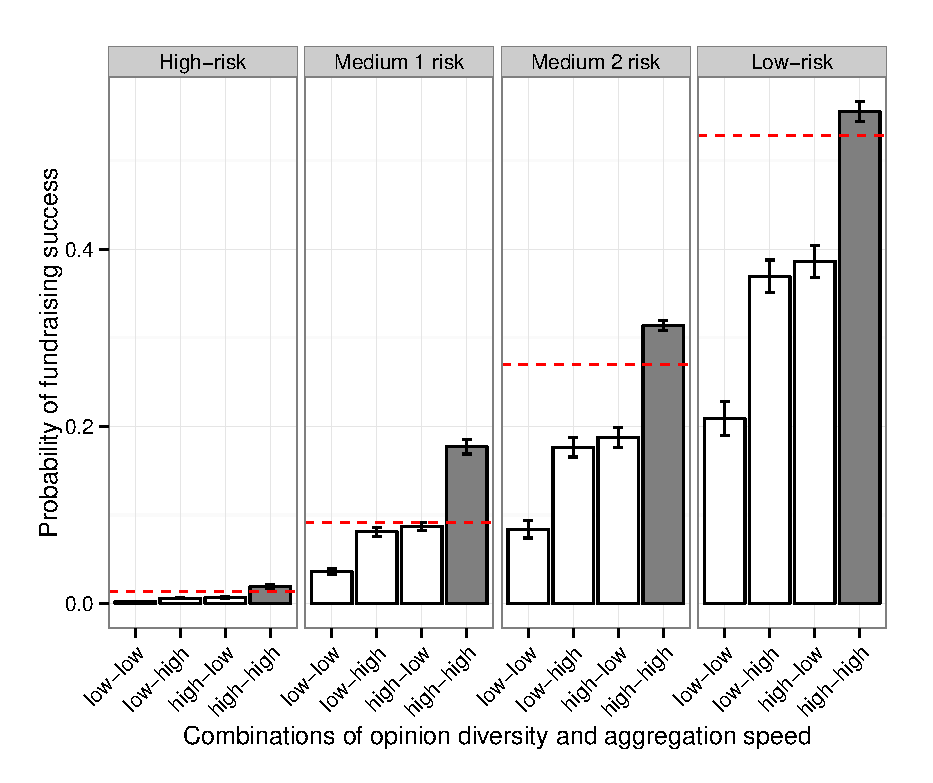
\epsfig{file=figs/FundedStata2.eps,width=0.45\textwidth,clip=}
    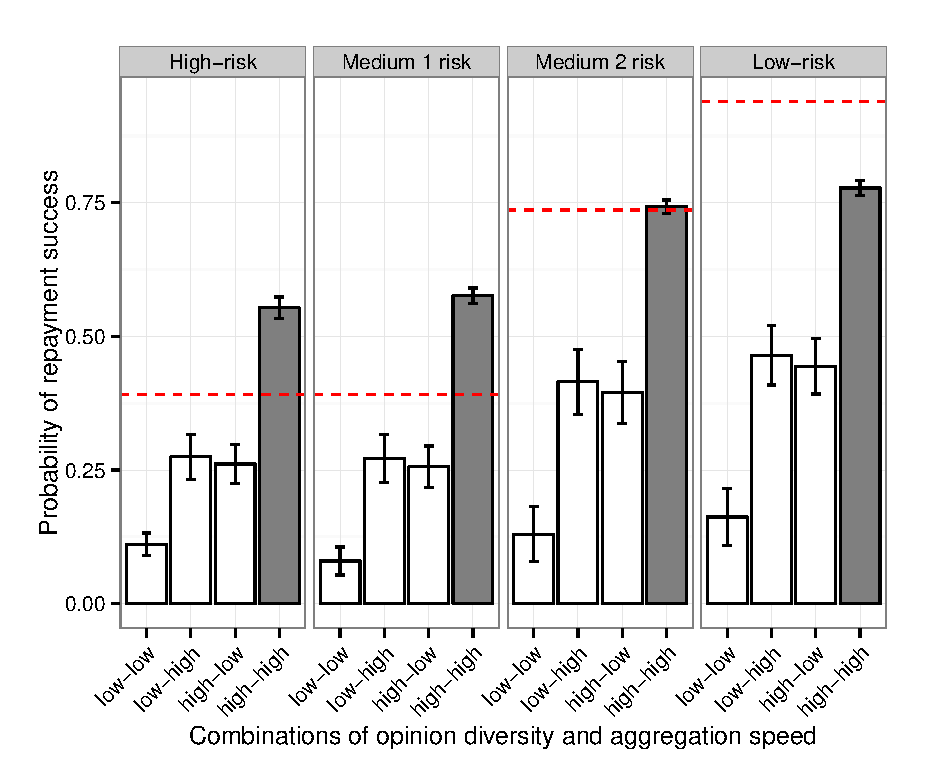
\epsfig{file=figs/RepaidStata2.eps,width=0.45\textwidth,clip=}
    \caption{Probability of successful fundraising (\emph{top}) and repayment (\emph{bottom}) for campaigns of different risk levels, conditional on opinion diversity and aggregation speed. Dashed lines indicate base rates computed under the assumption of random campaign outcomes in each risk category; gray bars depict the high opinion diversity and high aggregation speed condition that maximizes crowd wisdom. In seven out of eight cases, these campaigns are more likely to be successful than predicted by the base rate. Campaigns with a low diversity and/or aggregation speed perform worse than the base rate.}
    \label{fig:estimates}
    \vspace{-2em}
\end{figure}

Second, in all four fundraising risk categories (Figure~\ref{fig:estimates}, top panels), we see that the lift from crowd wisdom over the base is statistically significant. Even in the high-risk category, where the difference seems relatively small in real terms, the lift of the high-diversity and high-speed predictions is 37.6\%. The four repayment categories indicate the most interesting and important theoretical and practical findings from our study (Figure~\ref{fig:estimates}, bottom panels). The lift provided by crowd wisdom is statistically and substantially greater than expected by the base rate in the two categories with the highest risk. In the high-risk category, for example, the base rate estimates a repayment in roughly 40\% of the cases. In contrast, the combination of high diversity and high speed correctly predicts repayment 55.3\% of the time. 

Third, consistent with our hypotheses, we see that crowd wisdom consistently arises only when both diversity and speed are relatively high. Campaigns that are high on one but not both collective intelligence indicators have a success rate between 43.7\% and 95.2\% of the base rate, while campaigns that are low on both indicators (low diversity and low speed) have success rates up to 14.1\% lower than the base rate.

\paragraph{Collective intelligence indicators as early warning signals} Next we show that the two collective intelligence indicators of diversity and speed work reliably also with small crowds, suggesting that the crowdfunding system’s efficiency can be improved. To test the indicators' ability to predict fundraising success from a few bids relative to traditional measures of creditworthiness, we train a classifier at different bid numbers. We find that in the range of the first $k={1,2,...,10}$ bids, the random forest's performance in predicting fundraising increases from AUC=0.64 to AUC=0.76. With the increasing number of bids, the algorithm has more information about the progression of the bidding process, becoming more accurate.

Figure~\ref{fig:permutations} shows the permutation importance of the collective intelligence indicators relative to credit rating, debt-to-income ratio, and description length. Only 38.6\% of the campaigns receive more than 10 bids and thus lie outside of this analysis. As a validity check, we observe that for the minimum value of one bid, credit rating holds the most information about project merit. However, at four bids, opinion diversity and aggregation speed have more predictive value than credit rating. The importance of credit rating decreases over the bidding, while at the same time, the predictive power of diversity and speed grows. Note that the prediction accuracy of the random forests and the importance of the collective intelligence indicators relative to credit rating can be further elevated if the number of bids is included in an algorithm that learns based on all campaigns up to a given bid number. These findings indicate that diversity and speed are powerful in predicting borrower creditworthiness in populations of non-experts making complex estimates about future unknowns.  

\begin{figure}
    \centering
    \includegraphics[scale=.232]{samples/figs/permutations_lending.png}
    \caption{Collective intelligence indicators as early warning signals based on small crowds. Forecasts are made after each consecutive bid to assess prediction quality at the initial stages of campaigns. At the very beginning of the bidding process, credit rating is the most predictive variable. After only four bids, however, credit rating is outperformed by both opinion diversity and aggregation speed.}
    \label{fig:permutations}
    \vspace{-2em}
\end{figure}

\section{Discussion}
Several findings about dishonesty and corruption in the banking industry~\cite{Cohn2014,Villeval2014} highlight the challenges facing traditional financing models. At the same time, trends suggest that crowdfunding is growing at a rate that will possibly supplant traditional approaches from banks. Increased transparency, lack of financial intermediaries, and potential for diminished biases make crowdfunding an attractive alternative. Yet, little is known about how effective untrained crowds are at selecting creditworthy borrowers. Poor selection would misallocate funds from meritorious projects and possibly undermine the growth of crowdfunding systems.

Despite academic speculations about the ‘madness of crowds’~\cite{mackay2012extraordinary}, a few studies have shown that the consequences of violating some of the conditions for collective intelligence need not be as dramatic as suspected. For instance, research on prediction markets shows that crowd performance is superior to individual decisions even when individuals rely on the observable opinions of other crowd members~\cite{wolfers2004prediction,arrow2008promise}. Moreover, theoretical predictions and experimental results indicate that under certain conditions, influence among crowd members produces the most accurate judgments~\cite{becker2017network,almaatouq2020adaptive,beckerarxiv}.

Reliance on expertise also requires extensive experience or training, which can limit the supply of experts and diversity~\cite{uzzi1999embeddedness,Cohn2014}. For example, up until the early 1960s, it was accepted practice by bank loan officers in the United States not to consider women eligible for a loan unless their request was cosigned by a man~\cite{bystrom2018women}.  

In this paper, we contribute to the expanding literature on the wisdom of crowds with empirical evidence of a new form of collective intelligence that the crowd is not aware of. To do so, we apply concepts from the literature on the wisdom of crowds to examine whether factors that are thought to produce collective intelligence in other contexts operate in crowdfunding using a dominant crowdfunding platform. In agreement with theoretical expectations, we find that two collective intelligence indicators, i.e., opinion diversity and aggregation speed, quantified by the Gini coefficient of the bid amounts and the average inter-bid time, are predictive of who gets capital and who pays back. Furthermore, we find that these factors are potent at forecasting the outcome of high-risk campaigns and are indicative of successful fundraising, even in the early stages of a campaign.

Our results align with and advance work on the role of collective intelligence in crowdfunding. Others have shown recently that similar signals deduced from contribution patterns on various types of crowdfunding sites, including equity and donations-based platforms, are predictive of which projects will meet their fundraising goal~\cite{dambanemuya2021multi}. This work demonstrates associations between crowd dynamics and fundraising success in different contexts. Research relying on data from Prosper.com, specifically, points to various individual factors predicting default~\cite{serrano2015determinants,emekter2015evaluating,canfield2018determinants,iyer2015screening,dambanemuya2019harnessing}, albeit without properly accounting for the selection bias, i.e., the fact that we inherently lack the knowledge of whether an unfunded campaign would have returned the investment had it been funded. Furthermore, to the best of our knowledge, our paper is the first to show that lending crowds are (1) smart in the sense that they can predict the outcome of risky loans and (2) agile, meaning that they can concur on determinations of creditworthiness after only as few as four bids. Finally, recent experimental work further demonstrates the validity of similar collective intelligence indicators across a range of conditions, such as different project types, fundraising goals, participants' interest level in the projects, their altruistic attitudes, and their susceptibility to social influence~\cite{dambanemuyaarxiv}. 

The identified collective intelligence indicators are generalizable to many crowdfunding contexts (c.f.~\cite{dambanemuya2021multi} for predicting fundraising in newer datasets), simple to compute in any crowdfunding setting and distill key information from campaign dynamics. On the one hand, our indicators draw from the study of auctions, in that we focus on the amounts contributed as indicators of investors' assessment of borrower trustworthiness. Our derived concept of diversity is based on expressed opinions instead of predefined socio-demographic categories. In this regard, it is unique and one step ahead of traditional notions of diversity. On the other hand, our collective intelligence indicators exploit the temporal patterns emerging in crowdfunding by using accurate fine-grained data on campaign dynamics. Successful campaigns are characterized by lenders acting promptly, but not in unison, regarding bid amounts. The inequality of contributed capital observed in this study contrasts with hypotheses of irrational herding, which imply mimicry among lenders in risk-taking~\cite{Zhang2012}. We present evidence that even though its lenders do not act independently, Prosper.com gave rise to systematic crowd wisdom with tangible performance gains. This might help us to better understand and equip the future development of the crowdfunding phenomenon, which is of interest to organizations and governments. Our findings pinpoint the key component, which is central to human computation more broadly: latent collective behaviors that enhance crowd efficiency and lay the foundations for a crowd-aware system design.

\vspace{-1em}
\section{Conclusions}
Existing research on financing, both on- and off-line, has focused on characteristics of creditworthiness, such as credit scores~\cite{abdou2011credit,iyer2015screening}, social capital~\cite{Granovetter1985,uzzi1999embeddedness,Freedman2008,Greenberg2013,Lin2013,horvat2015network}, and the presentation of the borrower~\cite{Duarte2012,brooks2014investors,althoff2014ask}. These approaches lack a crowd-centric perspective and thus overlook the appealing possibility that Web-based crowdfunding might have produced conditions that have enabled the emergence of superior decision-making performance at the group level. Lending crowds benefit from aggregating multiple perspectives giving a more rounded view of the risk. However, crowd members are not independent and might be restricted by the actions of those who lend first, leading to cascading behavior that may not gravitate toward rational choices. Hence the two factors that could contribute to collective intelligence in crowdfunding are (1) the diversity of the perspectives in the lending crowd and (2) the aggregation mechanism that transforms individual evaluations into collective estimations considering that the decision-makers are not acting independently.

In this paper, we developed two collective intelligence indicators tailored to the specifics of crowdfunding. First, we looked at the inequality of loans, which directly polls the diversity of a group of lenders and overcomes the weaknesses of traditional categories such as gender, education, and ethnicity. Second, to devise a suitable aggregation mechanism, we studied the evolution of a campaign and viewed the time intervals between single bids as a particular combination of opinions that reinforces the crowd's overall assessment of the merit of a project. We then showed that our two resulting indicators, opinion diversity and aggregation speed, are predictive of campaign outcomes and can admit a model that jointly explains fundraising and subsequent repayment. Moreover, these indicators work particularly well with high-risk projects and might even serve as early warning signals of funding outcomes relying on data from small crowds. 

Altogether, our work has resulted in large-scale empirical evidence for collective intelligence indicators in online crowdfunding. These indicators have implications for lenders, borrowers, and platforms alike. Our findings call for more concerted digital literacy education for lenders about the positive and negative effects of crowd signals. Borrowers can improve the success of their campaigns, for example, by diversifying their outreach to multiple funder categories. Platform creators can develop higher-performing sites when harnessing collective intelligence indicators. Given that the indicators are heavily dependent on crowd activity, they could be manipulated by nefarious actors (c.f. how /r/wallstreetbets gamed the stock of GameStop~\cite{mendoza2021sticking}). Future research should therefore increase awareness of these collective intelligence indicators and investigate their robustness to potential manipulation. Finally, our findings contribute to the growing literature on collective intelligence and crowd computation, opening up new avenues for theoretical work inspired by the increasingly granular understanding of the surprising efficiency of Web-enabled wisdom of crowds systems.

\bibliographystyle{acm}
\bibliography{sample-base.bib}

\end{document}
\endinput
%%
%% End of file `sample-sigconf.tex'.
